% Spark refernce architectures
% Copyright (C) 2016 Jan Machacek
%
% This program is free software: you can redistribute it and/or modify
% it under the terms of the GNU General Public License as published by
% the Free Software Foundation, either version 3 of the License, or
% (at your option) any later version.
%
% This program is distributed in the hope that it will be useful,
% but WITHOUT ANY WARRANTY; without even the implied warranty of
% MERCHANTABILITY or FITNESS FOR A PARTICULAR PURPOSE.  See the
% GNU General Public License for more details.
%
% You should have received a copy of the GNU General Public License
% along with this program.  If not, see <http://www.gnu.org/licenses/>.
%

%%%%%%%%%%%%%%%%%%%%%%%%%%%%%%%%%%%%%%%%%%%%%%%%%%%%%%%%%%%%%%%%%%%%%%%%%%%%%%%%
%2345678901234567890123456789012345678901234567890123456789012345678901234567890
%        1         2         3         4         5         6         7         8

\documentclass[a4paper, 10 pt, conference]{IEEEtran}

\usepackage{graphicx}
\usepackage{interval}

\intervalconfig {
soft open fences ,
separator symbol =; ,
}

\title{Spark Reference Architecture \\ Sensor batch processing}

\author{Jan Machacek%$^{1}$% <-this % stops a space
%\thanks{Supported by Cake Solutions Limited}% <-this % stops a space
%\thanks{$^{1}$J. Machacek is the CTO at Cake Solutions, Houldsworth Mill, Houldsworth Street, Reddish, SK5 6DA, UK {\tt\small janm at cakesolutions.net}}%
}


\begin{document}

\maketitle
\thispagestyle{empty}
\pagestyle{empty}

%%%%%%%%%%%%%%%%%%%%%%%%%%%%%%%%%%%%%%%%%%%%%%%%%%%%%%%%%%%%%%%%%%%%%%%%%%%%%%%%
\begin{abstract}

TODO

\end{abstract}


%%%%%%%%%%%%%%%%%%%%%%%%%%%%%%%%%%%%%%%%%%%%%%%%%%%%%%%%%%%%%%%%%%%%%%%%%%%%%%%%
\section{Introduction}

TODO

\section{Reference implementation}

This architecture was used in a connected fitness application. The application processes inputs from one or more sensors (smartwatch, HR sensor, smart clothes) to track fitness regimes and to deliver targeted health and fitness advice to the users. 

The application on the user's smartphone connects data from the available sensors, combines it with a statistical model of the user's behaviour, and---where available---fine-grained location services. These three inputs allow the application to make the first distinction: exercise vs. no-exercise. From the user's perspective, the system is an automated fitness trainer; from a data scientist's perspective, the biometric data the system collects allows for detailed analysis of exercises, exercise regimes, impact of exercise on the users' well-being, automated physiotherapy, and many other applications.

\subsection{Architecture}

\begin{figure}[hb]
	\begin{center}
		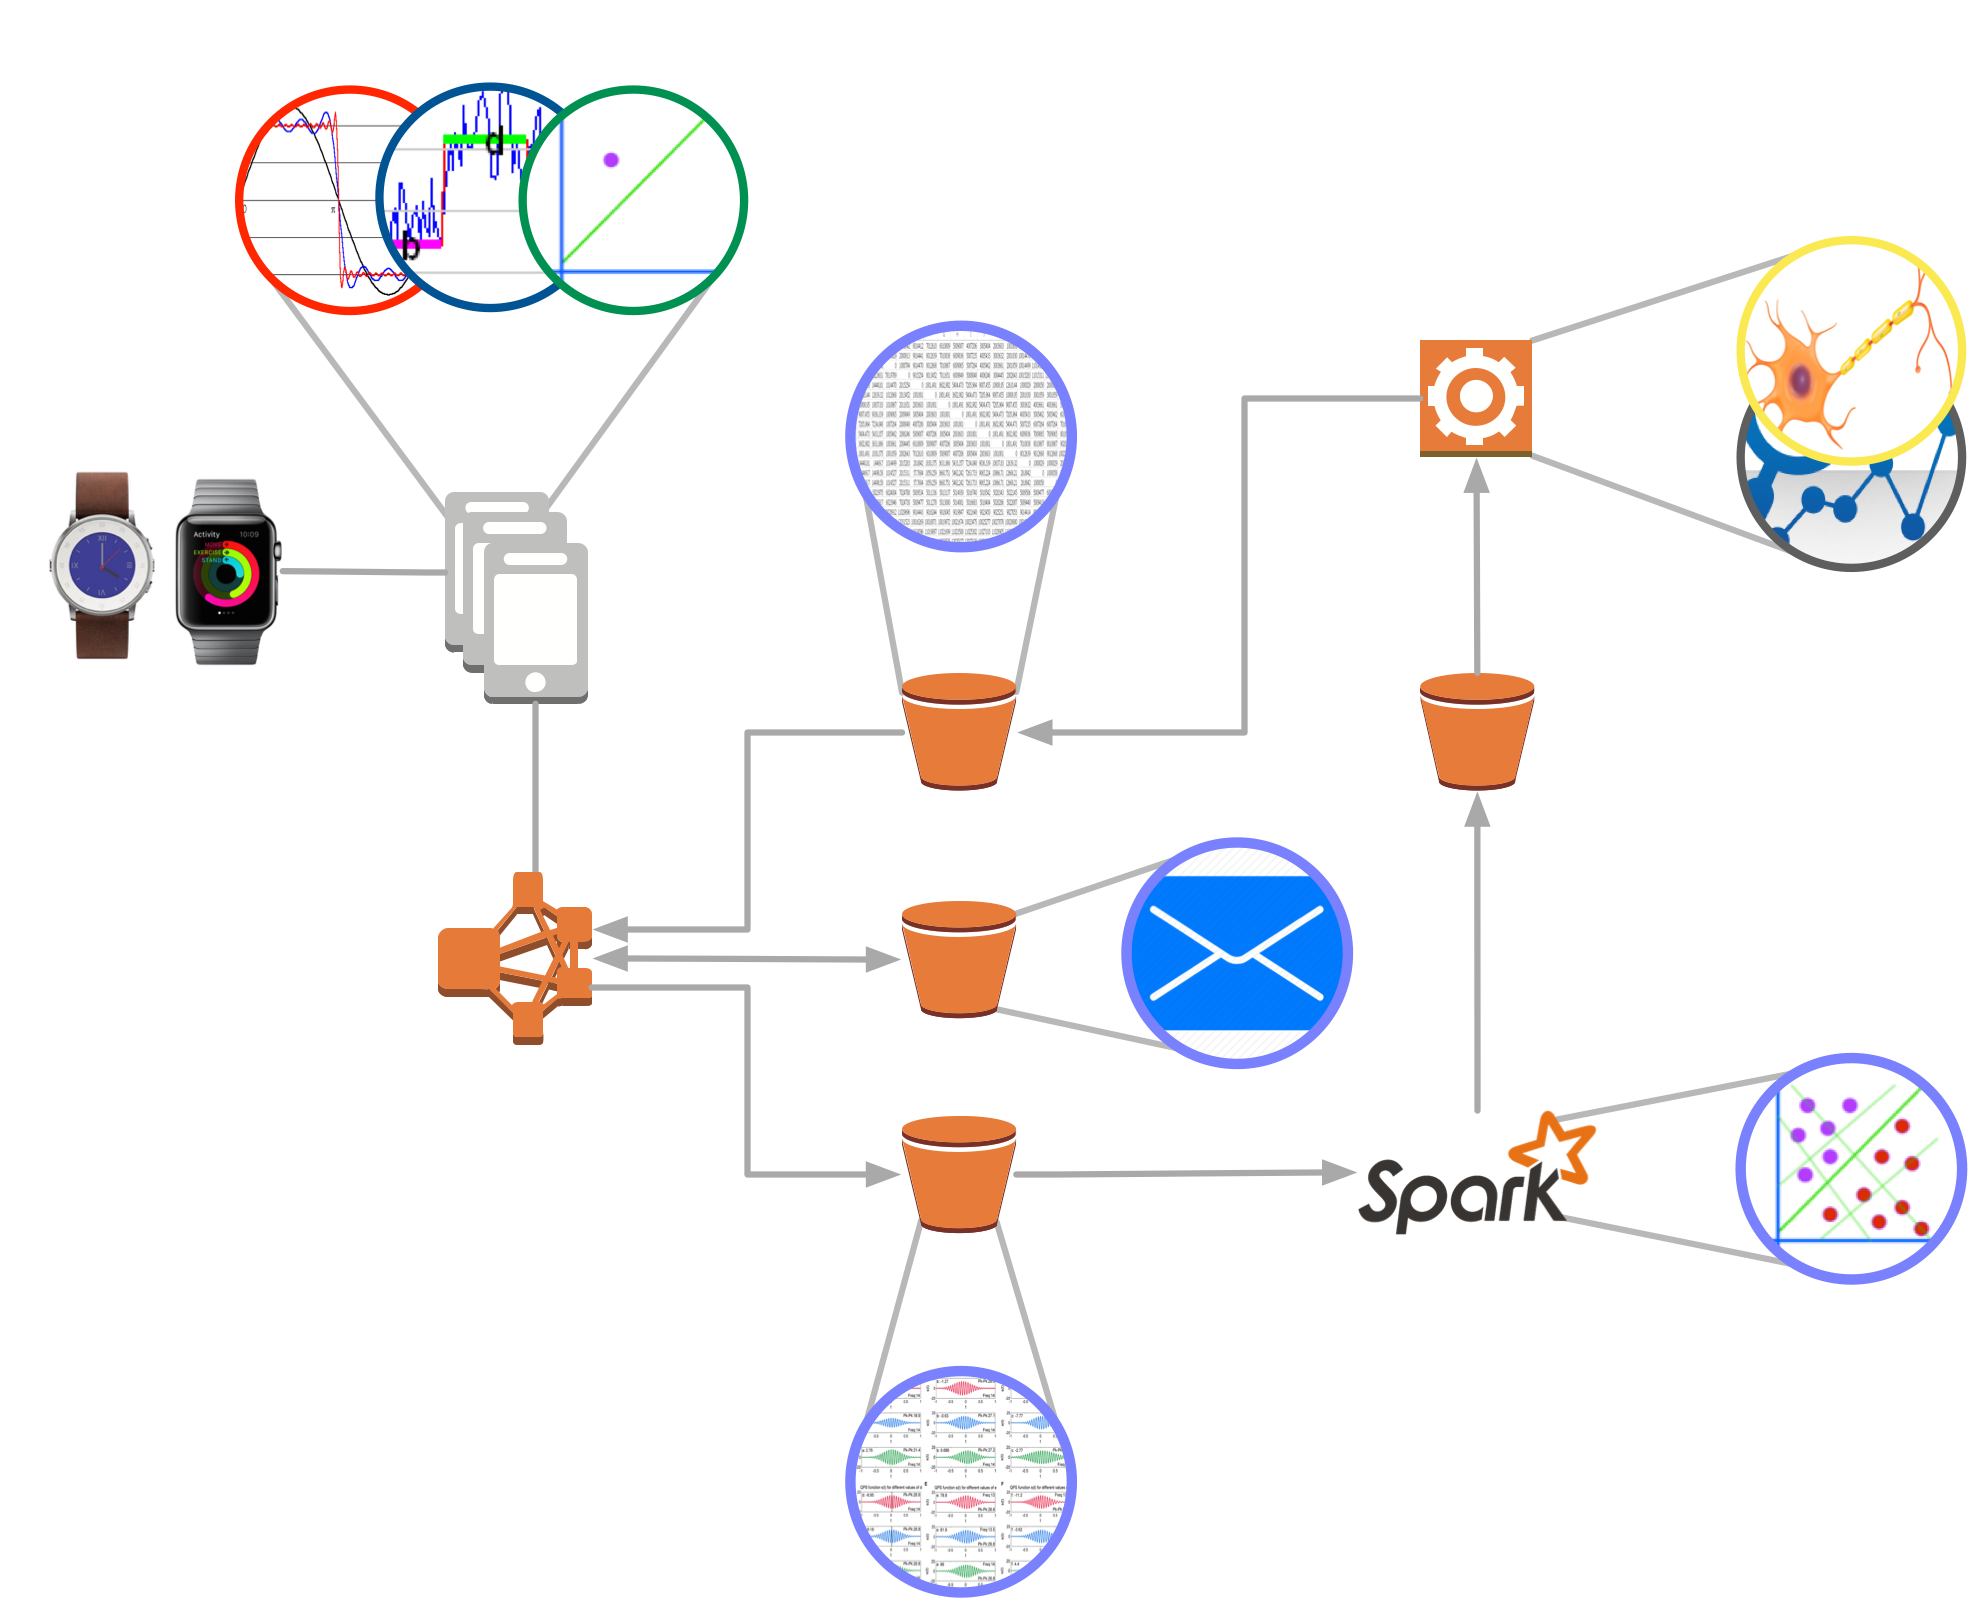
\includegraphics[scale=0.2]{ri-arch.png}
		\caption{Architecture}
		\label{default}
	\end{center}
\end{figure}

The sensors shown here as consumer-grade wearables perform only the basic hardware interaction: there is no pre-processing of the recorded data. The system accepts accelerometer, gyroscope, heart rate and---where available---data from strain gauges in smart clothes. The sensors send the data in 1s batches; the application on the mobile resamples the sampling rate to 50 Hz. (Accelerometer and gyroscope typically sample at this rate, heart rate and the strain gauges in smart clothes can be up-sampled to 50 Hz easily.) 

The sensor data in the mobile application is a set of vectors containing 1 second of input data of \texttt{float} values, normalised to a range of $\interval[open]{-1}{1}$ by using a maximum reasonable value for acceleration, rotation, strain and heart rate. (Looking at figure \ref{raw-acceleration}, one might consider $4 ms^{-2}$ to be such reasonable acceleration.)

\begin{figure}[hb]
	\begin{center}
		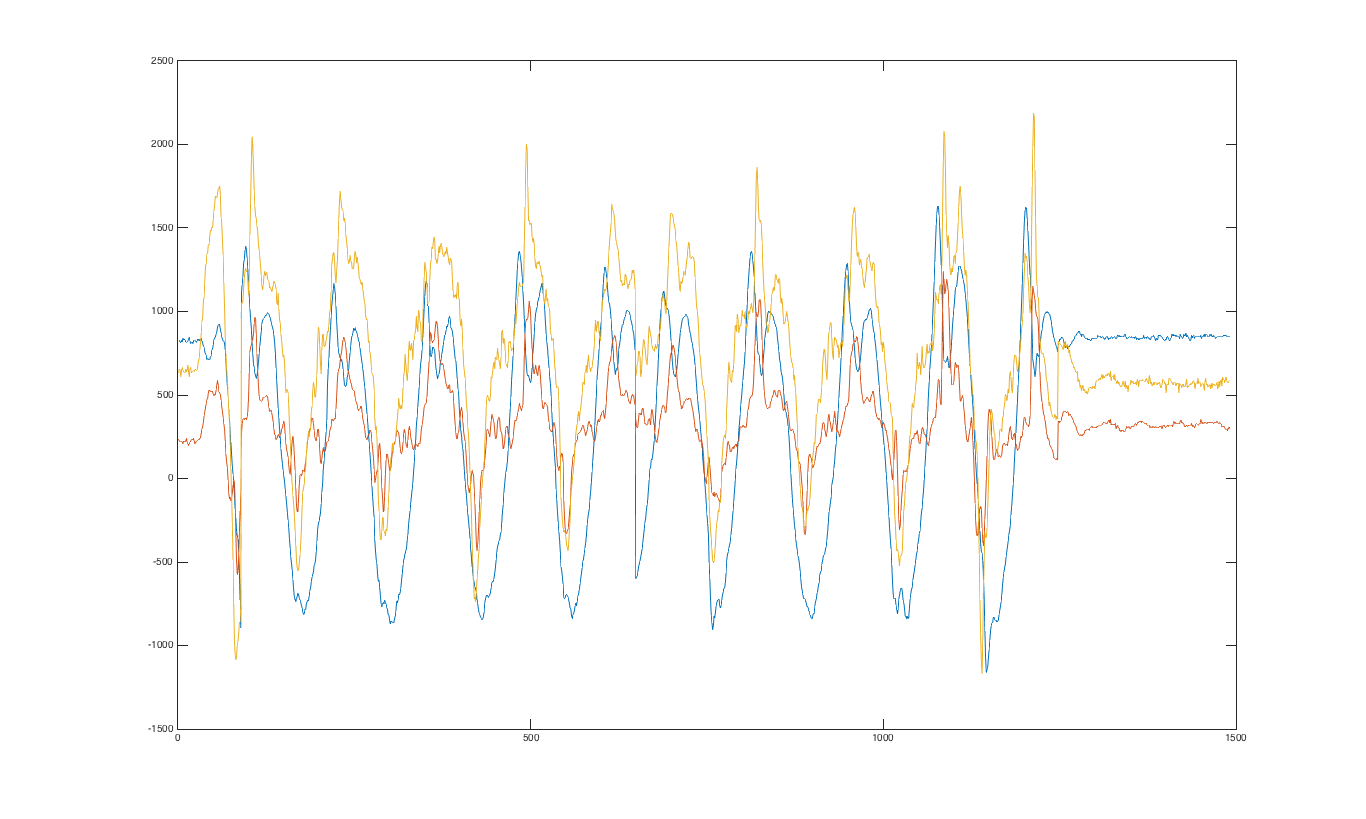
\includegraphics[scale=0.2]{ri-raw-acceleration.png}
		\caption{Raw acceleration data}
		\label{raw-acceleration}
	\end{center}
\end{figure}


It is important to realise that a single sensor input alone is not sufficient to accurately distinguish exercise from non-exercise. 

\begin{table}[h]
\caption{Evaluation of a CNN for exercise vs. non-exercise classification}
\label{exercise}
\begin{center}
\begin{tabular}{|c||c||c|}
\hline
Actual / Predicted & Exercise & Non-exercise\\
\hline
Exercise & 12330 & 2305\\
\hline
Non-exercise & 3542 & 13412\\
\hline
\end{tabular}
\end{center}
\end{table}

\section{Summary}

TODO

\addtolength{\textheight}{-12cm}  % This command serves to balance the column lengths
                                  % on the last page of the document manually. It shortens
                                  % the textheight of the last page by a suitable amount.
                                  % This command does not take effect until the next page
                                  % so it should come on the page before the last. Make
                                  % sure that you do not shorten the textheight too much.

\begin{thebibliography}{99}

\bibitem{c1} G. O. Young, ÒSynthetic structure of industrial plastics (Book style with paper title and editor),Ó 	in Plastics, 2nd ed. vol. 3, J. Peters, Ed.  New York: McGraw-Hill, 1964, pp. 15Ð64.

\end{thebibliography}


\end{document}
